\documentclass[tikz,border=10pt]{standalone}
\usetikzlibrary{calc}
\begin{document}
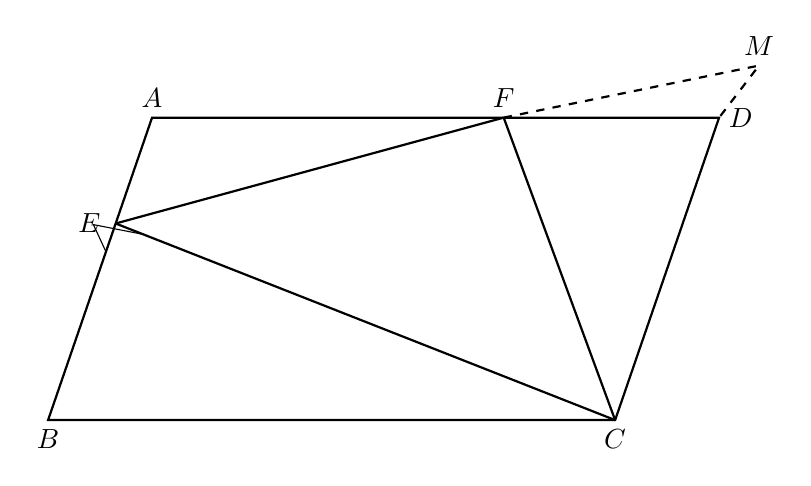
\begin{tikzpicture}[scale=1.2]
\coordinate (B) at (0,0);
\coordinate (C) at (6,0);
\coordinate (A) at (1.1,3.2);
\coordinate (D) at (7.1,3.2);
\coordinate (E) at ($(A)!0.35!(B)$);
\coordinate (F) at ($(A)!0.62!(D)$);
% M: perpendicular to AD at F, beyond D
\coordinate (M) at ($(F)+(2.7,0.55)$);
\draw[thick] (A) -- (B) -- (C) -- (D) -- cycle;
\draw[thick] (E) -- (C);
\draw[thick] (E) -- (F);
\draw[thick] (F) -- (C);
\draw[dashed,thick] (F) -- (M) -- (D);
% right angle mark at E between EB and EC
\draw ($(E)!9pt!(B)$) -- ($($(E)!9pt!(B)$)!9pt!90:($(E)!9pt!(C)$)$) -- ($(E)!9pt!(C)$);
\node[above] at (A) {$A$};
\node[below] at (B) {$B$};
\node[below] at (C) {$C$};
\node[right] at (D) {$D$};
\node[left=2pt] at (E) {$E$};
\node[above] at (F) {$F$};
\node[above] at (M) {$M$};
\end{tikzpicture}
\end{document}
